\documentclass[12pt,a4paper]{article}

\usepackage[margin=2.5cm]{geometry}
\usepackage[utf8]{inputenc}
\usepackage[brazil]{babel}
\usepackage{lmodern}
\usepackage{fancyhdr}
\usepackage{tocloft}
\usepackage{amsmath}
\usepackage{graphicx}
\usepackage{booktabs}
\usepackage{array}
\usepackage{float}
\usepackage{hyperref}
\usepackage{lastpage}
\usepackage{subcaption}

\graphicspath{{../../../imagens_gerais/} {puxamento/}} 

\pagestyle{fancy}
\fancyhf{} 
\setlength{\headheight}{30pt}
\lhead{
  \includegraphics[height=1.2cm]{lafe_logo_ingles.jpg} \\
  \small
  Doc ID: PLT0072 \quad
  Doc tipo: Relatório de fabricação \quad
}
\rhead{
  \small \textbf{PLT0072 Suspended core em PETG esverdeado} \\
  Page \thepage\ of \pageref{LastPage}
}
\lfoot{\small \textcopyright\ 2026 LaFE. All rights reserved.}
\rfoot{\small Última data de revisão: 28/05/2026}

\begin{document}

  Descrição da participação dos envolvidos na fabricação desta fibra:
  \begin{itemize}
    \item Eduardo Souza: Puxamento
    \item Ivan Prearo: Fabricação e puxamento
  \end{itemize}

  \section*{Puxamento}
  \label{sec:puxamento}

Este puxamento é de uma preforma do tipo suspended core com dimensões mostradas na Tabela \ref{tab:medidas_prefoma}. A preforma é mostrada na Figura \ref{fig:preforma}.

  \begin{table}[H]
    \centering
	  \begin{tabular}{ccc}	
		  \textbf{Medida} & \textbf{Medida absoluta [mm]} & \textbf{Medida relativa} \\ 
		\hline
		  Diâmetro externo & 15 & 1 \\
		  Espessura do clad & 3 & 0.2\\
		  Espessura das \textit{struts} & 0.6 & 0.04
	  \end{tabular}
	  \caption{Medidas na preforma.}
	  \label{tab:medidas_preforma}
  \end{table}

\begin{figure}[H]
	\centering
	
\includegraphics[width=0.5\linewidth]{images/Preforma.jpg}
	\caption{Foto da preforma antes do puxamento.}
	\label{fig:preforma}
\end{figure}


  Para realizar o puxamento utilizamos a rampa de temperatura descrita na Tabela \ref{tab:puxamento_rampa}.

  \begin{table}[H]
    \centering
      \begin{tabular}{c|c}
        \textbf{ [°C]} & \textbf{Tempo [min]} \\ 
        \hline
        60 & 60 \\
        80 & 15 \\
        100 & 5 \\
        110 & 2 \\
        \hline
        120 & 15 \\
        125 & 5 \\
        130 & 7 \\
        125 & 7 \\
        128 & 18 \\
        125 & 1 \\
        123 & 23
      \end{tabular}
    \caption{Rampa de temperatura antes e durante o puxamento. O puxamento começa na linha horizontal.}
    \label{tab:puxamento_rampa}
  \end{table}

  \begin{table}[H]
    \centering
	  \begin{tabular}{c|c}	
		\textbf{ [°C]} & \textbf{Tempo [min]} \\ 
		\hline
        60 & 60 \\
        80 & 15 \\
        100 & 5 \\
        110 & 2 \\
        \hline
        120 & 15 \\
        123 & - \\
	  \end{tabular}
	  \caption{Rampa de temperatura sugerida.}
	  \label{tab:nova_rampa}
  \end{table}

\section{Resultados}
\label{sec:resultados}

 Foram produzidos alguns metros de fibra com diâmetro externo entre 1 mm e 0.2 mm. Realizamos algumas microscopias para verificar a proporção da microestrutura na fibra final. Para isso, medimos as dimensões de cada atributo da fibra a fim de calcular a razão entre elas (Figura \ref{fig:secoes_transversais}).

  \begin{figure}[H]
    \centering
      \begin{subfigure}{0.45\textwidth}
      \centering
      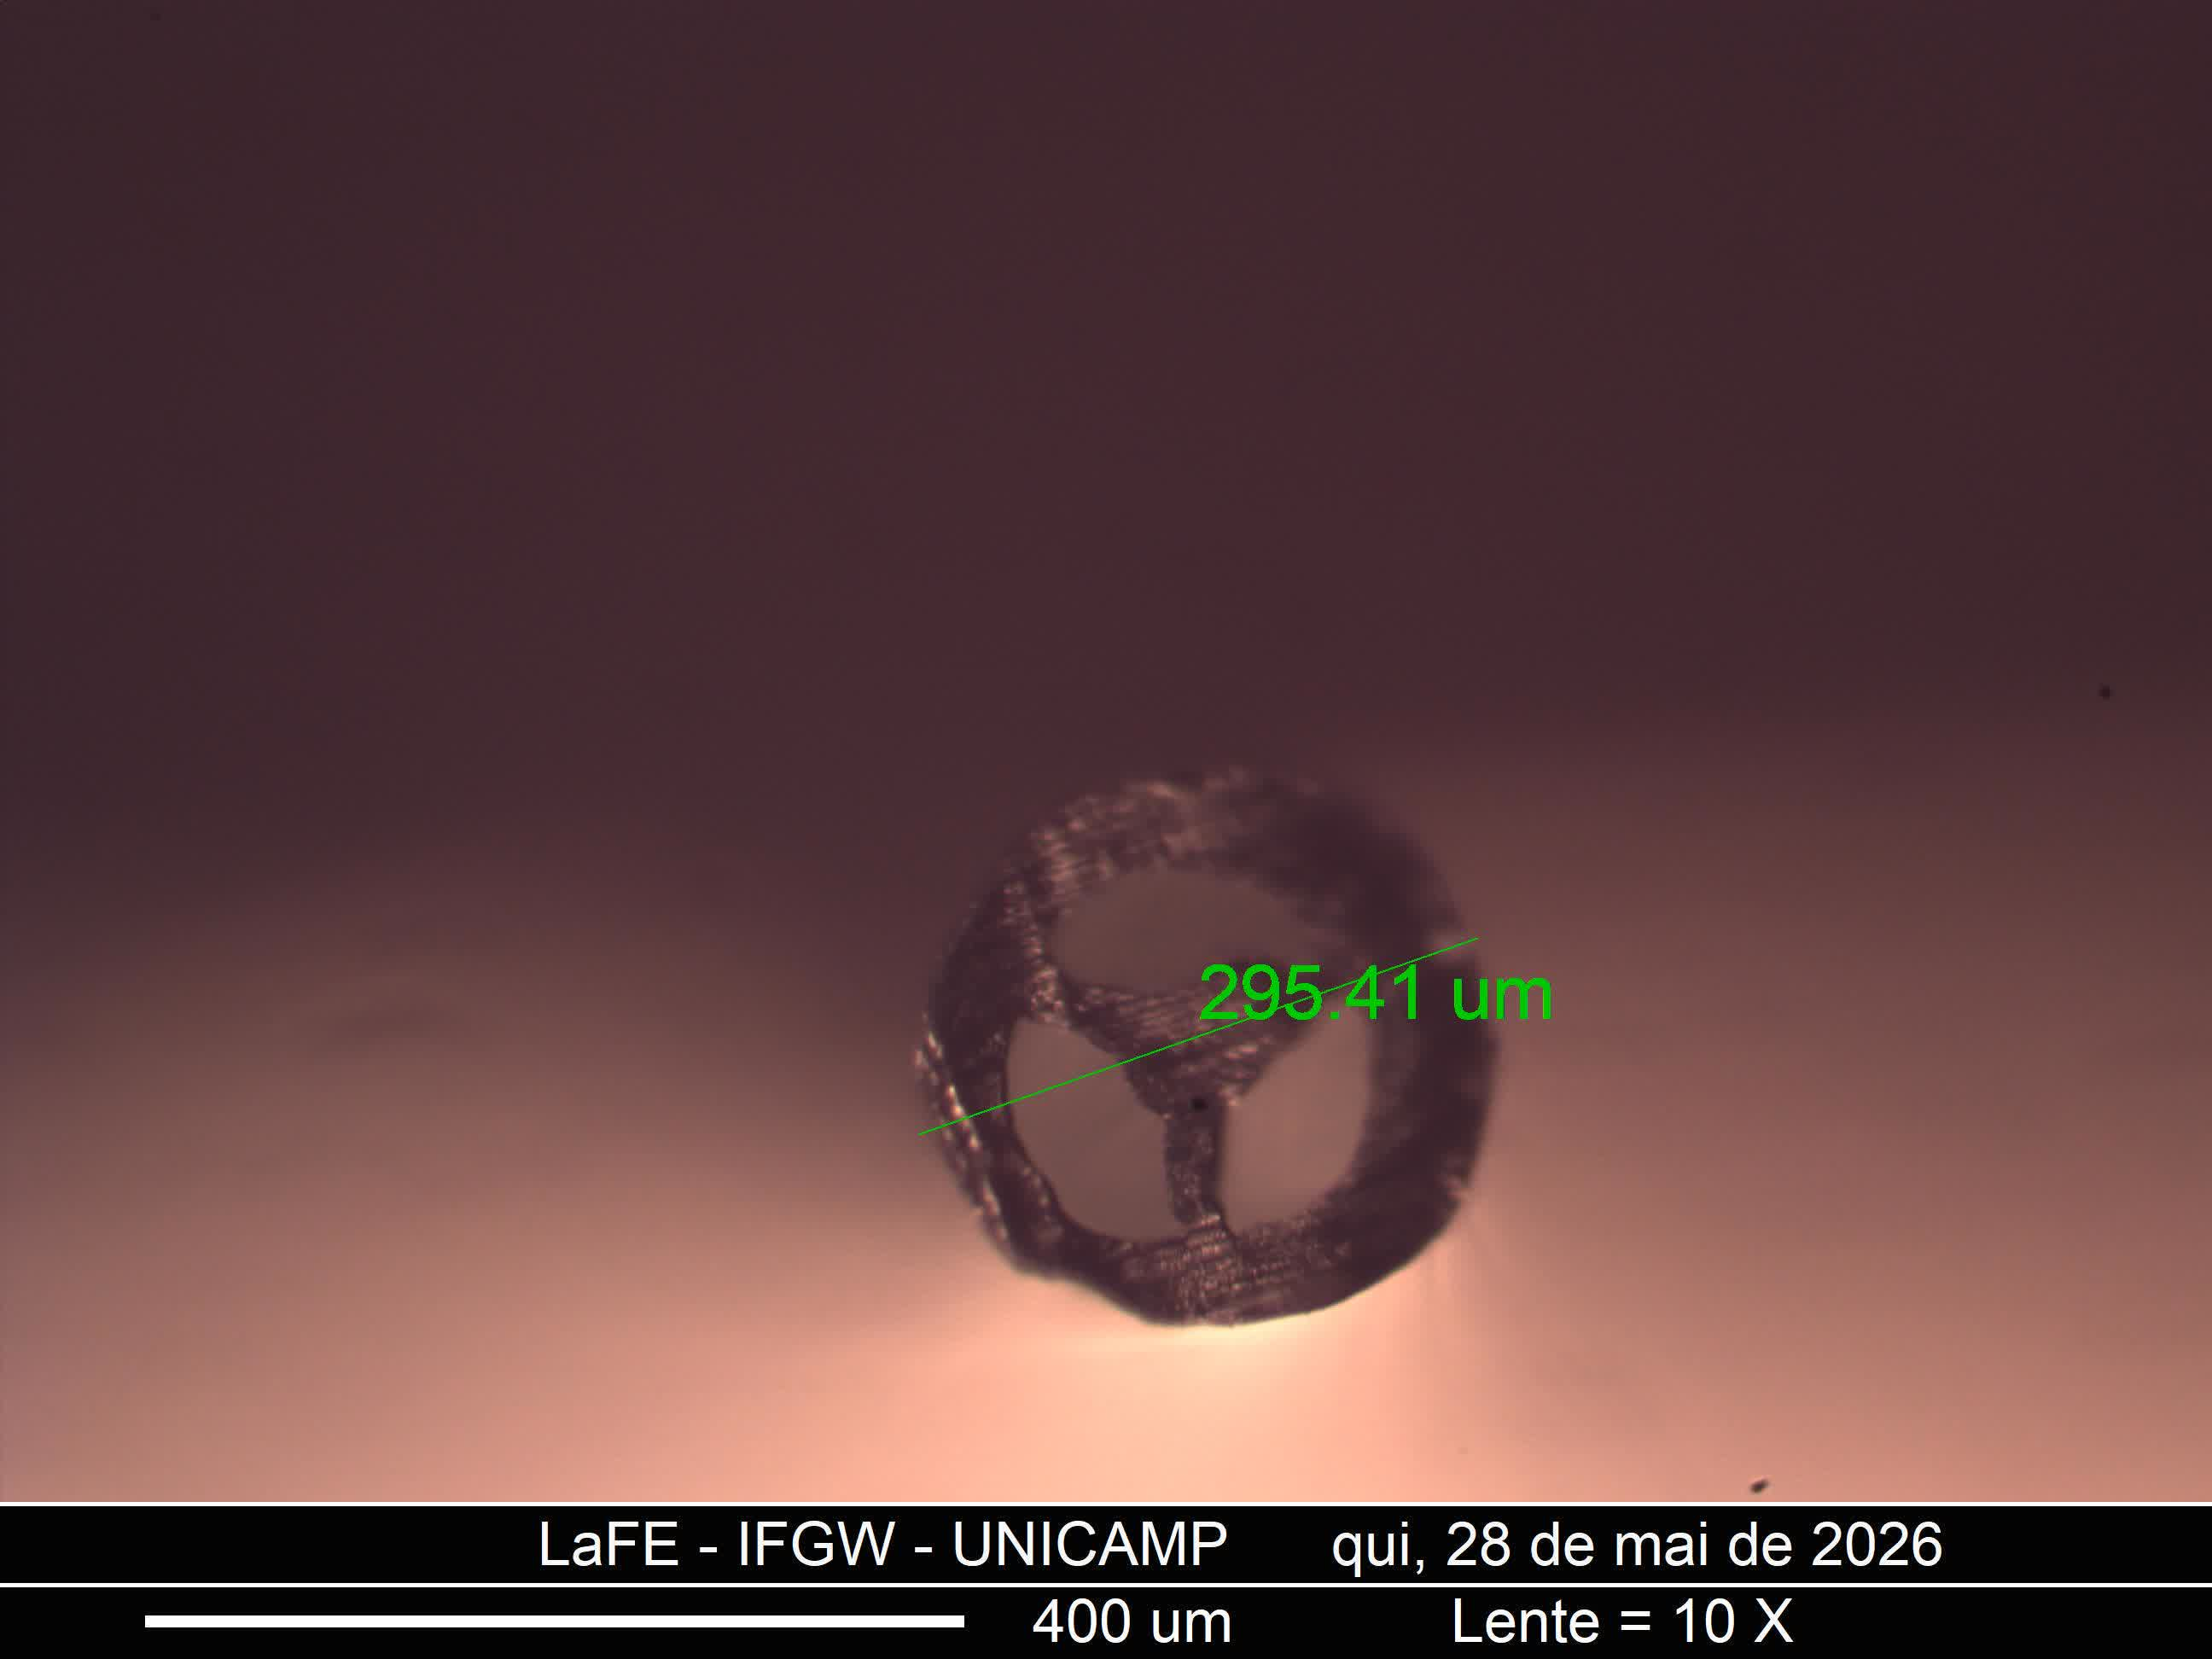
\includegraphics[width=1\linewidth]{images/F1_diam.jpg}
      \caption{Medida de diâmetro.}
      \label{fig:med_diam}
    \end{subfigure}
    \hfill
    \begin{subfigure}{0.45\textwidth}
      \centering
      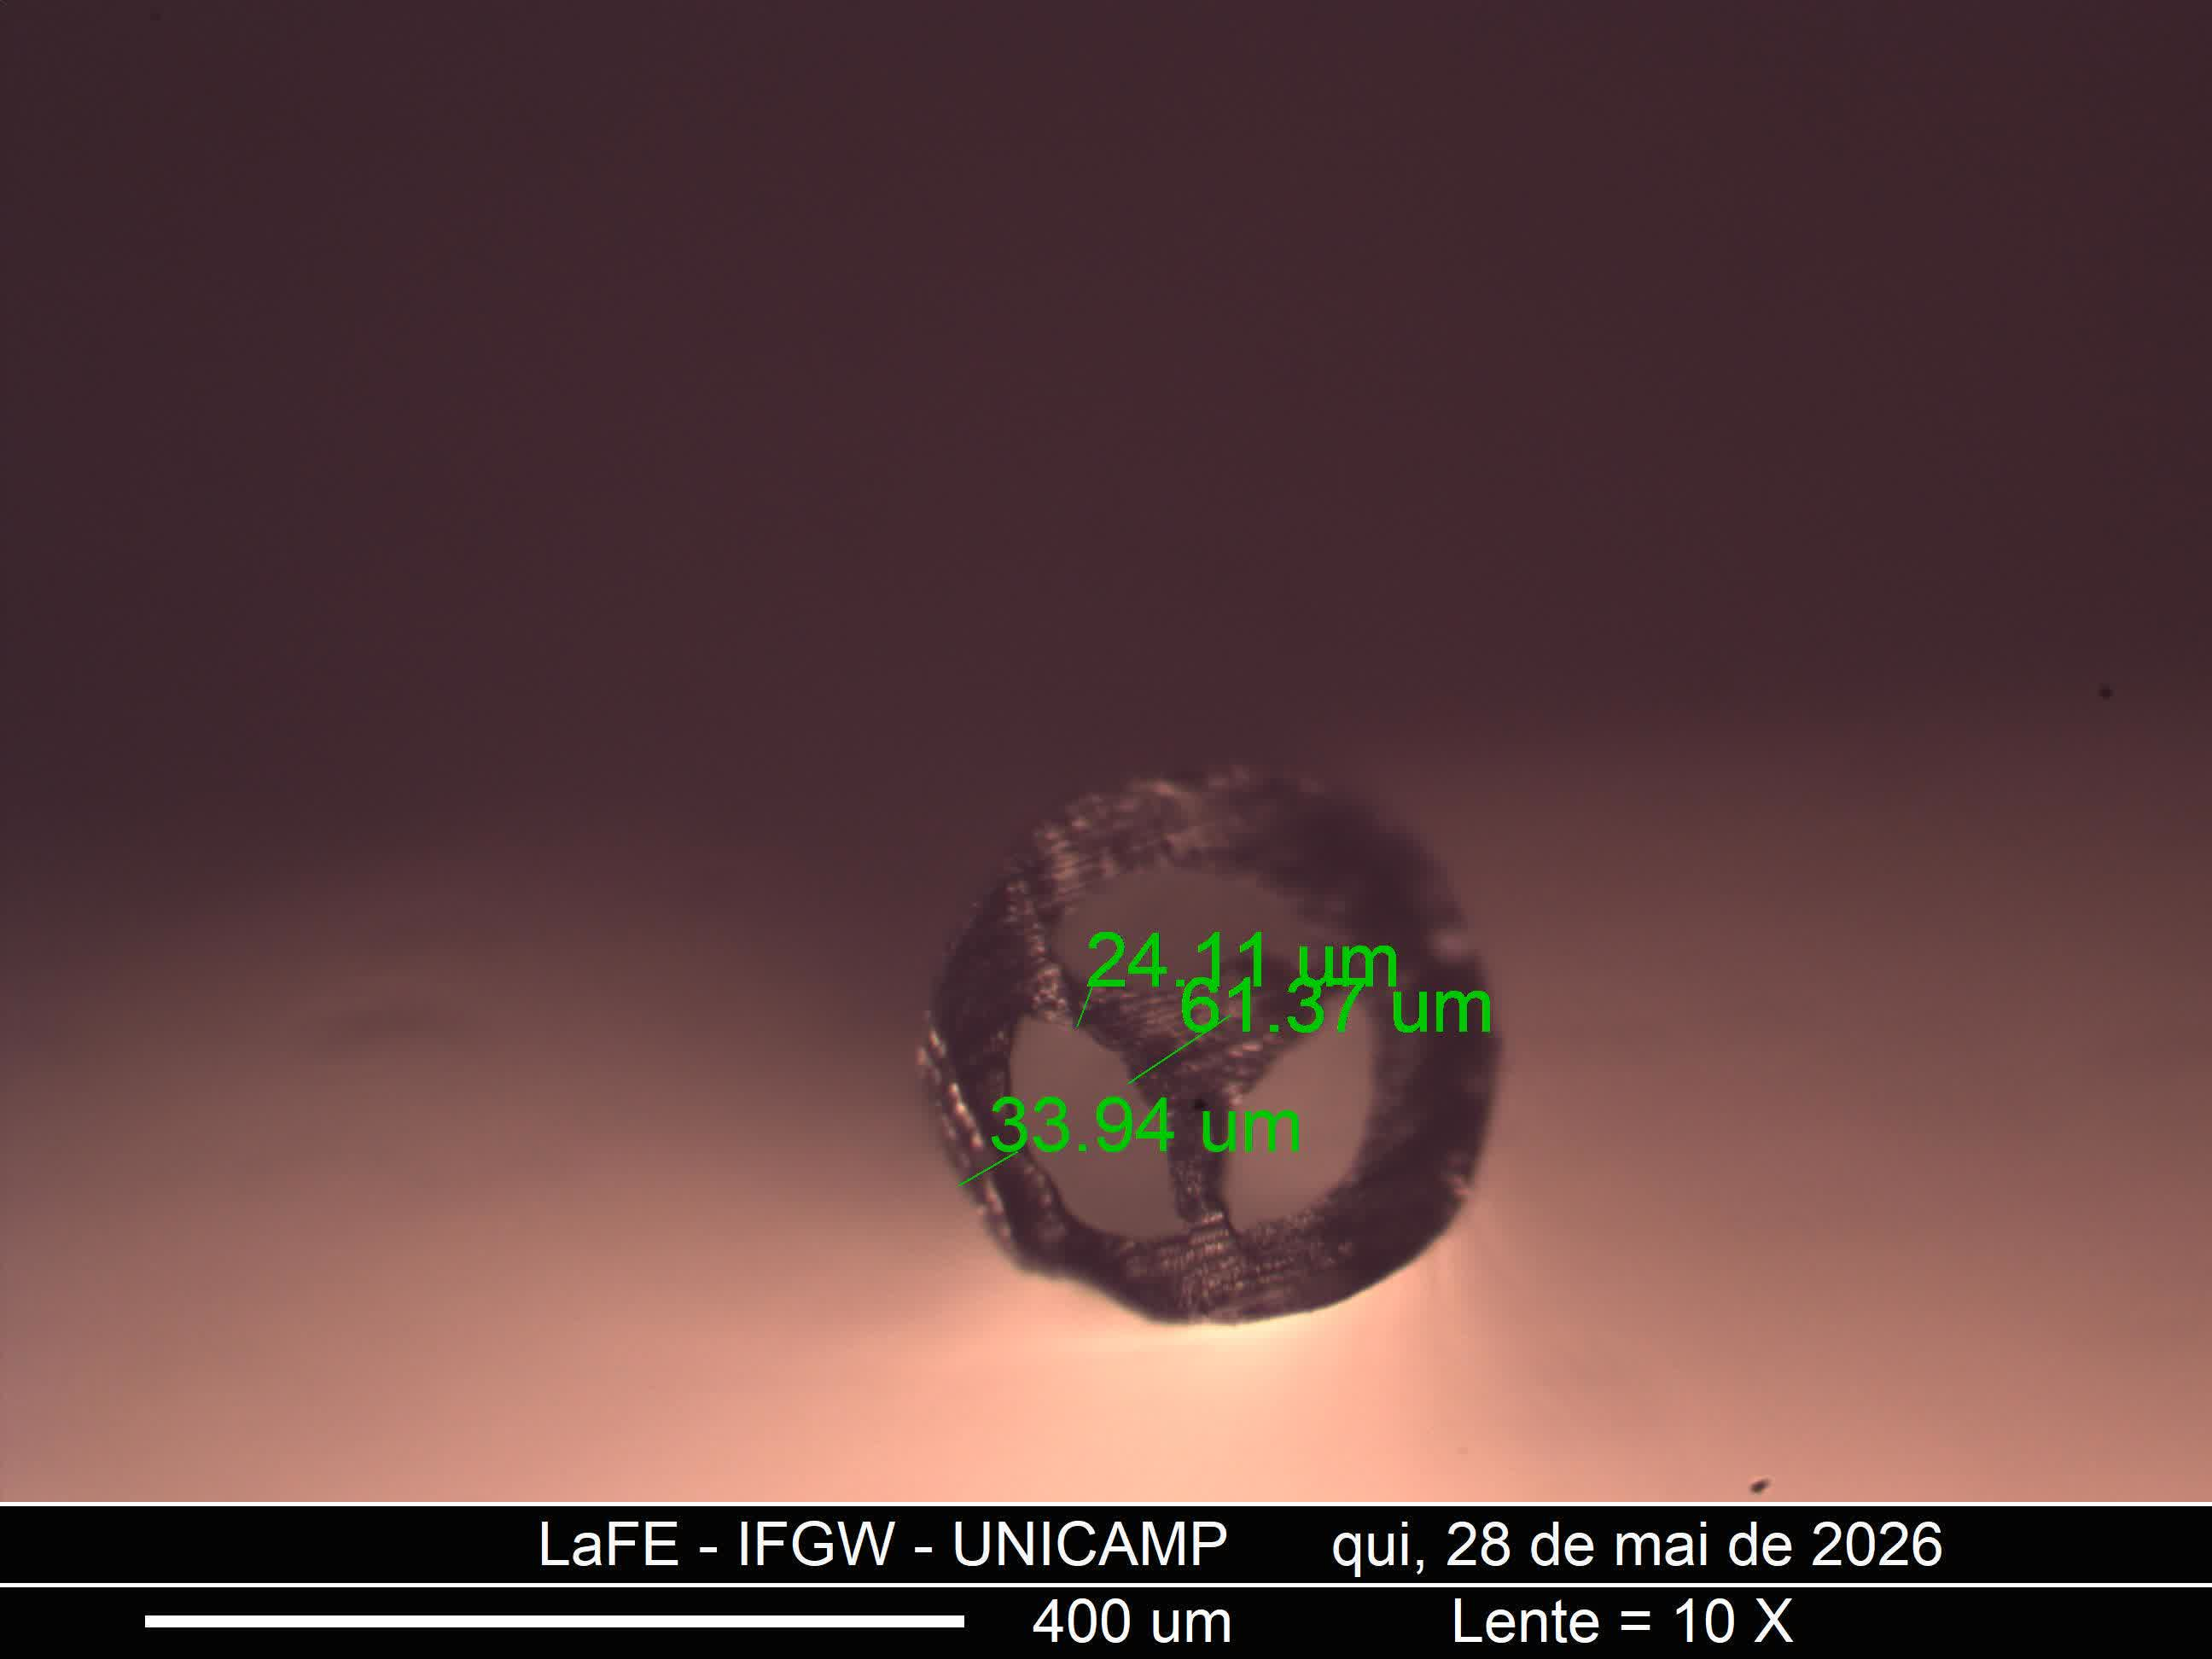
\includegraphics[width=1\linewidth]{images/F1_medidas.jpg}
      \caption{Medida de estrutura.}
      \label{fig:med_diam}
    \end{subfigure}
    \hfill
    \caption{Seção transversal da fibra analisada em microscópio.}
    \label{fig:secoes_transversais}
  \end{figure}


  \begin{table}[H]
    \centering
	  \begin{tabular}{ccc}	
		  \textbf{Medida} & \textbf{Medida absoluta [$\mu$m]} & \textbf{Medida relativa} \\ 
		\hline
		  Diâmetro externo & 295 & 1 \\
		  Espessura do clad & 34 & 0.115 \\
		  Espessura das \textit{struts} & 24 & 0.081
	  \end{tabular}
	  \caption{Medidas no final da fibra puxada (com pressão).}
	  \label{tab:fibra_final}
  \end{table}

\end{document}
